% !TEX encoding = UTF-8 Unicode
\documentclass{beamer}
\usetheme{CambridgeUS}
\setbeamercolor{bibliography entry author}{fg=black}
\setbeamercolor{item}{fg=darkred}
\setbeamercolor{caption name}{fg=darkred}

\usepackage{graphicx}
\graphicspath{{../Slike/}}
\usepackage[serbian]{babel}
\usepackage{type1ec}
\usepackage{cmap}

\newcommand{\autori}[4]{{\begin{tabular}{r l} #1 & #2\\ #3 & #4 \end{tabular}}}
\newcommand{\dvareda}[2][c]{\begin{tabular}[#1]{@{}c@{}}#2\end{tabular}}

\title{Paralelizacija metaheuristika}
\author[Mirkov, Vasović, Golubović, Heldrih]{\autori{Jovan Mirkov}{Lazar Vasović}{Dušica Golubović}{Teodora Heldrih}}
\institute[]{Matematički fakultet, Univerzitet u Beogradu\\\href{https://github.com/jvn-mirkov/Paralelizacija-metaheuristika}{github.com/jvn-mirkov/Paralelizacija-metaheuristika}}
\date[Matematički fakultet]{28. april 2020.}

\begin{document}

\frame{\titlepage}

\begin{frame}{Sadržaj}
\tableofcontents[subsectionstyle=hide]
\end{frame}

\section{Optimizacija i paralelizacija}
\subsection{Optimizacioni problemi}
\begin{frame}{Optimizacioni problemi}
\begin{itemize}
\item Optimizacija -- odabir najboljeg rešenja

\item Problemi -- ciljna funkcija i skup ograničenja

\item Egzaktno rešavanje -- iscrpna pretraga

\item Heuristike -- približna usmerena pretraga

\item Metaheuristike -- opšte strategije pretrage
\end{itemize}
\end{frame}

\subsection{Može li bolje?}
\begin{frame}{Može li bolje?}
\begin{itemize}
\item Sekvencijalne metaheuristike nekad nezadovoljavajuće

\item Paralelizacija -- mogućnosti paralelnog izvršavanja

\item Performanse -- brzina izvršavanja, robusnija rešenja

\item Podela posla -- podaci (naredbe), zadaci (jedinice)

\item Fizički nezavisni uređaji -- distribuirani algoritmi
\end{itemize}
\end{frame}

\subsection{Paralelne metaheuristike}
\begin{frame}{Paralelne metaheuristike}
\begin{itemize}
\item Dizajn -- arhitektura algoritma

\smallskip\small
\begin{tabular}{| c c c c |} \hline
Granularnost & \dvareda{Zavisnost\\od problema} & Ponašanje & Cilj\\ \hline
Nivo algoritma & Nezavisan & Izmenjeno & Efektivnost\\
Nivo iteracije & Nezavisan & Neizmenjeno & Efikasnost\\
Nivo rešenja & Zavisan & Neizmenjeno & Efikasnost\\ \hline
\end{tabular}

\medskip\normalsize
\item Implementacija -- arhitektura sistema

\smallskip\small
\begin{tabular}{| c c |} \hline
Arhitektura & Predstavnici\\ \hline
Programabilna kola & FPGA kola\\
Višeprocesorski sistemi & Višejezgarni sistemi, GPGPU\\
Distribuirane platforme & Klasteri, P2P, grid, oblak\\ \hline
\end{tabular}
\end{itemize}
\end{frame}

\section{Unapređivanje populacije jedinki}
\subsection{Strategije i modeli}
\begin{frame}{Unapređivanje populacije jedinki}
\begin{itemize}
\item Sekvencijalni algoritam evolucije zahteva velike računarske resurse
\item Paralelizacija kao posledica nezavinosti jedinki u populaciji
\item Strategija paralelizacije
\begin{itemize}
    \item paralelizacija populacije
    \item paralelizacija operacija
\end{itemize}
\item Primena -- problem Štajnerovog drveta u telekomunikacijama
\item Gospodar-sluga model
\item Struktuirana populacija
\end{itemize}
\end{frame}

\subsection{Struktuirana populacija}
\begin{frame}{Struktuirana populacija}
\begin{figure}
    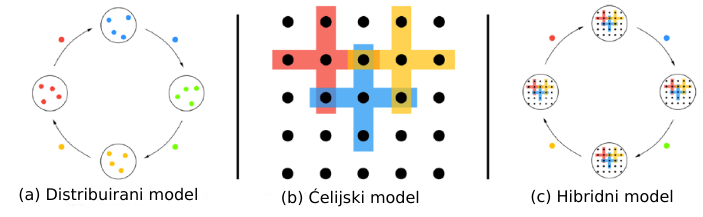
\includegraphics[scale=0.6]{struktuiraniModeli.png}
    \caption{Grafički prikaz distribuiranog, ćelijskog i hibridnog modela}
\end{figure}
\end{frame}

\subsection{Planovi migracija}
\begin{frame}{Planovi migracija}
\begin{itemize}
\item Distribuirani model -- planovi migracija
\begin{itemize}
    \item razmak između migracija
    \item stopa migracije
    \item odabir i zamena jedinki
    \item topologija (definisanje susedstva)
\end{itemize}
\item Model sa nezavisnim pokretanjima

\end{itemize}

\end{frame}

\section{Unapređivanje jednog rešenja}
\subsection{Ideja i primena}
\begin{frame}{Unapređivanje jednog rešenja}
\begin{itemize}
\item Osnovna ideja -- pretraga i zamena rešenja 

\item Zamena zavisi od konkretne metode

\item Prve ideje o paralelizaciji ovih algoritama oko 1980. godine

\item Primena -- GRASP algoritam za problem pouzdanosti u telekomunikacijama

\end{itemize}
\end{frame}

\subsection{Modeli paralelizacije}
\begin{frame}{Modeli paralelizacije}
\begin{figure}
    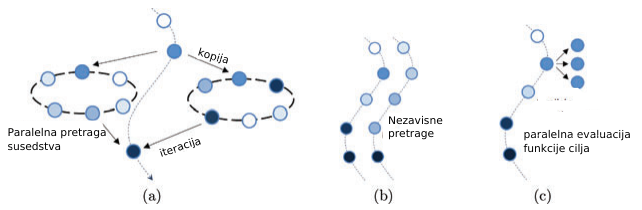
\includegraphics[scale=0.6]{albaPodela.PNG}
    \caption{\dvareda{Modeli paralelizma prema Enrikeu Albi: (a) kretanje,\\(b) višestruko pokretanje, (c) ubrzano kretanje}}
\end{figure}
\end{frame}

\section{Zaključak i literatura}
\subsection{Prednosti i izazovi}
\begin{frame}{Zaključak}
\begin{itemize}
\item Prednosti paralelizacije
\begin{itemize}

\item ubrzanje izvršavanja metaheuristika

\item bolji kvalitet rešenja

\item problemi sa većim dimenzijama

\item ograničenja
\end{itemize}

\item Izazovi paralelizacije
\begin{itemize}
\item najbolje rešenje

\item najbrže rešenje
\end{itemize}
\end{itemize}
\end{frame}

\subsection{Zahvalnica}
\begin{frame}
\centering \LARGE
\textbf{HVALA NA PAŽNJI!}

\textbf{Pitanja?}
\end{frame}

\subsection{Literatura}
\begin{frame}{Literatura}
\nocite{*}
\bibliographystyle{amsalpha}
\bibliography{SM_14_Prezentacija_ParalelizacijaMetaheuristickihAlgoritama_MirkovVasovicGolubovicHeldrih}
\end{frame}

\end{document}